% Tuning and temperament chapter
\chapter{Tuning and Temperament}

The topic of tuning and temperament is one of the most well-documented and
discussed issues in music.  I cannot produce any new information on this subject that
has not already been produced.
For our own understanding, however, there should follow a
concise summary of tuning and temperament as they are used in the context of
this paper. What follows is a short history of western tuning methods and
systems of temperament.  Because there are so many different kinds of
temperaments, I will only concentrate on the types that will be used for
discussion and comparison later.  These main types are modern-day equal
temperament and other temperaments with equal semitones, the regular meantone
temperaments known as quarter-comma and sixth-comma meantone, and the tuning
systems attributed to Pythagoras and Ptolemy.

The majority of my information comes from well-known and documented sources.
First and foremost in this area is Murray Barbour's 1951 book \textit{Tuning and
Temperament: A historical survey} as well as more recent books such as Ross
Duffin's \textit{How Equal Temperament Ruined Harmony (and why you should
care)}.  As the latter title suggests, discussions of temperament usually
revolve around the concept of equal temperament and whether or not its purpose
is justified during certain periods of music history.  Barbour's book, while
considered one of the most thorough compendiums of information, generally
portrayed temperaments other than equal temperament as inferior. Authors such as
Duffin and others in the historical performance field feel that equal
temperament has degraded the effect of musics for which it was not originally
intended.  Furthermore, Barbour relies heavily on the unit of cents in his
comparisons of temperaments, a unit which derives its significance from equal
temperament.  I choose to avoid using cents and compare temperaments in terms of
the ratios as well as using scaled drawings that show differences in terms of
fret distance.

It is my aim to fall on neither side of these debates regarding the use
of equal temperament in any music, modern or early.  Instead, I wish to remain
``temperament agnostic'' and let the historical sources speak for themselves,
using their own original ratios as their mathematical representations.
Varieties of equal temperament that relied on the equal division of the
semitone certainly did exist in the sixteenth and seventeenth centuries;
however their use was discouraged because of the consequences to harmony.
Consequences aside, use of such temperaments did find favor with fretted
instruments, which is the topic that this paper addresses.

\section{The Greeks' debate}

The history of tuning begins with the ancient Greeks and their philosophers
who proposed the first solutions to tuning notes within the span of an
octave.  Three of the most influential figures in this area were Pythagoras,
Aristoxenus and Claudius Ptolemy. Pythagoras is generally credited with
discovering the concept of tuning, although none of his original writings
survive.  He established the first mathematical principles that apply to
tuning; however, it was Aristoxenus and Ptolemy that began the debate about
tuning which is still continues today.  One of the fundamental teachings of the
Pythagoreans was that the universe could be explained according to simple
numbers and ratios.  An example of this numerical simplicity is found in the
tetractys, a common symbol associated with the Pythagoreans because it
represented the basic sequence of numbers: 1, 2, 3, and
4.  Pythagoreans believed that everything in the world could be reduced to these simple
numbers.
% Pythagorean tetractys
\begin{figure}[h]
\centering
\setlength{\unitlength}{1mm}
\begin{picture}(30,30)
% bottom row = 4
\put(0,0){\circle*{2}}
\put(10,0){\circle*{2}}
\put(20,0){\circle*{2}}
\put(30,0){\circle*{2}}
% second row = 3
\put(5,10){\circle*{2}}
\put(15,10){\circle*{2}}
\put(25,10){\circle*{2}}
% third row = 2
\put(10,20){\circle*{2}}
\put(20,20){\circle*{2}}
% top row = 1
\put(15,30){\circle*{2}}
\end{picture}
\caption{The Pythagorean tetractys}
\end{figure}
The number four, for example, could be used to explain the four seasons of the
year or the four elements of earth, wind, fire and water while the sum of the
numbers (1 + 2 + 3 + 4) gave you 10 and that was the basis for their entire
system of arithmetic.\autocite[273]{CN:1} For the Pythagoreans, numbers meant
everything.

Today, such notions of numeric significance are usually found in
numerology and astrology.  To us, such associations seem almost nonsensical because we are taught
a more scientifically developed understanding of the universe; however,
basic mathematical principles of number underpin even our most complex theories.
To regard the Pythagoreans' notions of number and meaning as absurd belies
the fact that our notions of meaning are tied to same kinds of numbers, but just
in a different way.  For them, just as much as us today, everything operated
according to numbers and music was no exception.

Historically, Pythagoras discovered how numbers affected the tuning of musical
notes by listening to the hammers of blacksmiths.  According to the story, he
heard two blacksmiths each wielding hammers of different sizes.  The pitch that
each made when striking the anvil produced a musical interval.  He determined
that the type of interval produced depended on the weight ratio of the two
hammers. A hammer that was twice as heavy as another hammer would produce an
interval of an octave.  Whether or not the story is true, Pythagoreans expressed
tuning in terms of these kinds of ratios.

For the Pythagoreans, the most important intervals were the unison, octave,
fifth and fourth.  Not only were these the first pitches in the harmonic series,
but you could also express them using very simple numeric ratios: 1:1 for the
unison, 2:1 for the octave, 3:2 for the fifth and 4:3 for the fourth.  Because
these numbers fit perfectly into the Pythagorean notion of the teractys, any
other intervals in a scale ultimately had to be derived from these original
four, regardless of what the actual pitches were in reality.\autocite[274]{CN:1}
In other words, the music did not matter, it was only about the math.  The math
could be translated into music in different ways. The most common was the
monochord, which was a single string divided into different parts.  In order to
produce the intervals in a Pythagorean tuning system, the monochord was divided
into a certain number of parts and then stopped with either a finger or small
bridge.  For example, to produce an octave with the ratio 2:1, the monochord was
divided into two parts and stopped at the first part. For the perfect fifth with the
ratio 3:2, it was divided into three parts and stopped at the second
part.  Other intervals were calculated by a combination of subtraction or
addition of the original four intervals.  In terms of arithmetic, the sum of two
ratios meant a product of the two, while subtraction of two ratios meant using
division.  So a Pythagorean would calculate a wholetone by subtracting the
fourth from the fifth.
\begin{equation}
3:2 \div 4:3 = 9:8
\end{equation}
This produced a wholetone with a ratio of 9:8. A semitone was then
calculated by subtracting two of these wholetones from the original fourth.
\begin{equation}
    (4:3 \div 9:8) \div 9:8 = 256:243
\end{equation}
This produced a ratio of 256:243. Of course these ratios were not part of the
tetractys, but that did not matter because the resulting semitone was created from intervals
that were.  In this case, the fourth, already a member of the original four
intervals, and the wholetone created from the fourth and fifth.

While the numerical simplicity of using only unisons, octaves, fifths and
fourths fit perfectly with the Pythagorean ideal, using them as the basis for a
tuning system produced unacceptable results when applied in a musical context.
Tuning an entire scale using only Pythagorean ratios created several problems,
the first of which was that the system was not internally consistent.  We can tune a chromatic
scale using only Pythagorean fifths by starting with the interval C to G and continuing through
the circle of fifths for all twelve pitches, returning the the original note C.
\begin{figure}[h]
\centering
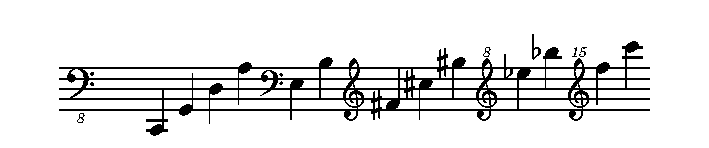
\includegraphics{examples/12-fifths.pdf}
\caption{The circle of twelve fifths}
\end{figure}
After proceeding through twelve fifths from our starting C, the final C is seven octaves above it.
\begin{figure}[h]
\centering
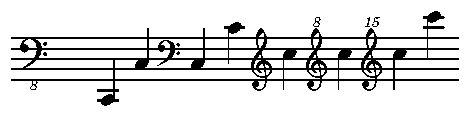
\includegraphics{examples/7-octaves.pdf}
\caption{The note C spanning seven octaves}
\end{figure}
If Pythagorean tuning was internally consistent, the C seven octaves above would be the
exact same pitch as the C resulting from twelve fifths.  We can test this mathematically,
by adding together twelve ratios of 3:2 and comparing them with the sum of seven octaves
using the ratio 2:1.\autocite[25]{RD:1}
\begin{equation}
    \frac{3}{2} \times
    \frac{3}{2} \times
    \frac{3}{2} \times
    \frac{3}{2} \times
    \frac{3}{2} \times
    \frac{3}{2} \times
    \frac{3}{2} \times
    \frac{3}{2} \times
    \frac{3}{2} \times
    \frac{3}{2} \times
    \frac{3}{2} \times
    \frac{3}{2} = \frac{531441}{4096} = 129.7463
\end{equation}
\begin{equation}
    \frac{2}{1} \times
    \frac{2}{1} \times
    \frac{2}{1} \times
    \frac{2}{1} \times
    \frac{2}{1} \times
    \frac{2}{1} = \frac{128}{1} = 128
\end{equation}
The mathematical result is that the sum of the twelve fifths is greater than the sum of the
seven octaves.  In musical terms, the C resulting from twelve fifths is sharper
than what we expect to hear, a C seven octaves above the C from which we started.

Pythagorean tuning presented another problem as well.  Not only was it not internally consistent
but was that it was not consistent with the rest of the harmonic series either.
The first three pitches in the harmonic
series matched Pythagorean ratios perfectly.  The pure intervals of the octave,
fifth and fourth in the harmonic series were exactly in tune when compared to the
ratios of their Pythagorean counterparts. However, the fourth pitch in the
harmonic series, the major third, when tuned acoustically pure as it naturally
occurred in the series, actually vibrated at a ratio of 5:4 and not
81:64, as the Pythagoreans would have calculated by adding together two of
their 9:8 wholetones: $ 9:8 \times 9:8 = 81:64 $.

These two tuning discrepancies that result from using only Pythagorean intervals
to build a scale of notes are called \textit{commas}.  The \textit{ditonic comma}
results when building a chromatic scalle upon successive fifths,
such as the difference between twelve fifths
and seven octaves, and the \textit{syntonic comma} results when trying to match the
Pythagorean major third and the pure harmonic major third.  The
Pythagoreans themselves were well aware of these problems and tried to overcome them, but it
was only Aristoxenus and Ptolemy that could propose any real solutions.
Aristoxenus proposed a solution by ignoring the Pythagorean ideals of
mathematical simplicity and used tuning systems that divided the string
according to parts and not ratios.  He described tuning by using equal parts of
the string and was the first to develop the concept of tuning using equal
semitones which would later be the foundation of equal temperament.  Ptolemy on
the other hand continued with the Pythagorean notion of ratio, except he modified
it slightly.  In Ptolemy's view, tuning should only use ratios that are
superparticular in nature, meaning that the first number of the ratio should
always be one unit great than the other.  So Pythagorean ratios like 2:1, 3:2, 3:4
and even 9:8 were acceptable, but so too were other ratios such as 5:4, the pure
major third and 6:5, the pure minor third.

Ptolemy's solution rectified a lot of the Pythagoreans' mathematical
ratios with nature's own internal tuning system but it still had problems when it came to
musical execution.  In a twelve-tone scale, there are three major thirds. Starting
on the note C, we can fit three of them within an octave:
C to E, E to G-sharp, and A-flat to C.
\begin{figure}[h]
\centering
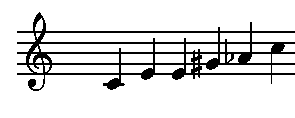
\includegraphics{examples/thirds.pdf}
\caption{Three major thirds within an octave}
\end{figure}
However, adding these intervals together using Ptolmey's
ratios does not get us to a complete octave either.  The sum of three thirds should sound
the same as an octave with the ratio 2:1, but the mathematical result it slightly less than
2, which sounds flat.
\begin{equation}
    \frac{5}{4} \times
    \frac{5}{4} \times
    \frac{5}{4} \times = \frac{125}{64} = 1.953125
\end{equation}
While the note E could remain fixed in relationship to the major third starting
from C and the major third ending on G-sharp, the fact that G-sharp and A-flat
are used for the other two major thirds implies that they are different notes.
Most modern musicians regard the enharmonic respelling of a note as a kind of
music homonym: an alternative word to express the same thing.  While the
different names of G-sharp and A-flat can indicate different functions, such as
the third degree of the E major scale or the first degree of the A-flat major,
we today regard them as notes having the same vibrating pitch.
However, as Ptolemy's tuning problem shows us, the two notes are not only
functionally different, they are musically different are therefore tuned differently.

Ptolemy's solution of tuning with only pure intervals is known as just intonation.  While
it succeeded in correcting the problems associated with Pythagorean tuning, it made it impossible
to tune certain notes in the chromatic scale because they required a different tuning depending on
musical context in which they occurred.  Instruments of fixed pitches,
such as any keyboard instrument or fretted instrument, whose semitones
were fixed and immobile, could not accommodate a tuning of only pure
intervals, or at least, not in a scale of twelve tones.  Instruments
of variable pitch, such as any bowed instrument, wind instrument or
the human voice were exempt from this problem because they were able
to adjust any note sharper or flatter depending on the need of the
situation.  A violinist, for example can place his or her finger
on the fingerboard of the instrument in any position as well as a
wind player that may vary the pitch of a note with his of her
embouchure.

What about Aristoxenus?  While he did invent an alternative solution of equal
semitones, he rejected both the notions of Pythagorean numeric purity and the
Ptolemaic notion of harmonic purity.  His method of tuning divided an octave
into equal parts, making intervals as groups of these individual parts instead
of using ratios at all.  It was his idea of equal parts that former the basis for
equal temperament.  While this allowed for a tuning of fixed pitches in a chromatic scale,
none of these intervals were tuned in a way that precisely matched the tuning in the harmonic
series.  For most theorists and musicians during the history of western
classical music, this was an unacceptable solution, and it took many years for
us to finally embrace the idea of equal temperament.

Because the notion of equal semitones did not sit well with early western music
theorists and tuning harmonically pure intervals was impossible in a fixed pitch
system, they gravitated towards the Pythagoreans' system of tuning.  For one
reason, it was simple and operated using the idea of small number of simple
ratios.  For another reason, it matched the musical tastes of the medieval
period such as monophonic chants and polyphonic forms based on fifths, unisons
and octaves.  Pythagorean ratios persist even to this very day, but as music
changed in the early Renaissance period, composers sought to incorporate more
consonant thirds into their music, which the strict Pythagorean system of ratios
did not easily accommodate.  Thus, the old Greek debate between Pythagoras,
Ptolemy and Artistoxenus resurfaced again.

\section{Temperament}

For most of the Middle Ages, tuning was described according to the same
ratios that Pythagoras had determined hundreds of years earlier. However, as
musical tastes changed during the Renaissance, there was an increasing
preference for the sounds of thirds instead of unisons and fifths. This
represented the problem of rectifying thirds within the Pythagoran tuning
scheme that had plagued the Greeks so many years before. The solution
to the problem was to change the size of the fifth within the Pythagorean
system.

Tempering is a process of compromise where the acoustical purity of one interval
is changed slightly in order to accommodate the acoustical impurity of another
interval.  Generally speaking, it is the process of changing the size of the fifth in
order to accommodate the major third which is not pure within the standard
Pythagorean tuning. Usually this means shrinking the size of the fifth slightly
so that is narrower, or flatter than the pure ratio of 3:2, although in some
cases, a fifth may be tuned wider or sharper than pure. The problem with
Pythagoran thirds were that they were much sharper than pure, differing by the
syntonic comma which was the difference between the Pythagorean third at 81:64
and the pure harmonic third at 5:4. Shrinking the size of the fifth resulted in
thirds that were flatter than the Pythagorean ratio of 81:54 and closer to the harmonically
pure ratio of 5:4, and thus tolerable
in a musical context.  Depending on the amount in which you flattened the fifth, you
could achieve a pure 5:4 third, but at the expense of a very out-of-tune fifth.  The
strategy was to shrink several fifths by the same or differing amounts. The result
was that instead of one set of intervals being completely pure in nature and
another being completely out-of-tune and unusable, all the fifths were slightly out-of-tune
in differing amounts, while some of the thirds came very close to pure.

Murray Barbour classifies temperaments into four basic types: regular meantone,
irregular temperaments, equal division, and equal temperament. Whereas
a tuning can be defined as a method of obtaining intervals according to
Pythagoras, as in Pythagorean tuning, or according to Ptolemy, as in
just intonation, temperaments alter the ratios of the intervals so
that they are often somewhere in between the two systems. In regular
meantone temperaments, most or all of the fifths of the Pythagorean tuning system
are tuned flat by the same amount.  Depending on the amount in which the fifths are
flattened, this can result in thirds that are very close to
to pure; however, the fifths and fourths are always not pure.  The amount
that each fifth was changed from its pure ratio often depended on the
musical context.  A meantone temperament that tuned fifths very flat
resulted in a temperament that had thirds quite close to pure, but
because of the mutated nature of the fifths, was only playable in
a limited number of keys.  Conversely, a meantone temperament that
tuned its fifths less flat made more keys playable,
but resulted in sharper, less pure thirds.

\subsection{Regular Meantone and Irregular Temperaments}

No one is entirely sure who invented the first complete meantone temperament,
but the general consensus is that it is a shared prize between Pietro Aron and
Gioseffo Zarlino.  Barbour credits Franchinus Gafurius's \textit{Practica
musica} of 1496 with the first mention of the idea of temperament.  In it,
Gafurius says that organists tune their fifths slightly flat, but does not go
into any specific details.\autocite[25]{MB:1}  Similarly, Arnolt Schlick's 1511
treatise \textit{Spiegel der Orgelmacher und Organisten} only gives us a general
idea when he refers to tuning the fifths only flat "as much as the ear will
permit." \autocite[202]{RR:1}  So it seems the idea is present as early as the
end of the 15th century, but it has yet to become a system.  Zarlino
gets the credit for an exact system that narrows each fifth by $\frac{2}{7}$ of a syntonic
comma.  While his method is exact--and he even provides a monochord diagram
of it as well--tempering the fifths by that much actually creates thirds that
are smaller than pure, or too flat.

Pietro Aron is credited with the first practical meantone temperament.  While
not as theoretically exact as Zarlino's, Aron's instructions can be used to
create a workable meantone temperament that narrows fifths enough to create pure thirds, while
leaving the remainder of the intervals playable.  His instructions are not mathematical in
nature, unlike Zarlino's, and requires the person to tune according to the
ear and not rely on measurements.  Aron's idea was to start with pure thirds and build
tempered fifths around them.  He begins with a pure third between C and E
and then proceeds to tune four fifths that are all equally flat with additional pure thirds
between A and C-sharp, and D and F-sharp.  While Aron says nothing about the division of
the comma, Barbour takes these instructions and mathematically proves that
if the tuner is able to create Aron's pure thirds by ear and match the size
of the other fifths so that they are all tempered by the same amount, each
of those fifths will be flatter than pure by $ \frac{1}{4} $ of a syntonic
comma.\autocite[27]{MB:1}  Because this is the measurable amount that each fifth is reduced
in size, this Aron's temperament is referred to as ''$ \frac{1}{4} $ Meantone temperament``.
While Aron never called his temperament this, nor did he use any math to calculate lengths of
a string, theorists and musicians took his ideas and later produced exact calculations that
reproduced Aron's temperament.

Regular meantone temperaments contained a number of fifths that were all narrowed by
the same amount. This was always measured in terms of a fraction of the syntonic comma.
Narrowing four consecutive fifths in the circle of fifths by $ \frac{1}{4} $
of a syntonic comma was enough to make eight thirds in a 12-tone scale pure while leaving the
remaining four practically unplayable.\autocite[33]{RD:1}  This was an
effective solution for sixteenth-century music which did not make use
of the keys in which these unplayable thirds resided.  Furthermore,
quarter-comma meantone also created a ``wolf'' fifth that was too wide to be used.
Again, this still was acceptable because the fifth was not used.

Due to the problems that quarter-comma presented with wolf fifths and other
thirds that were unplayable, other tuning systems appeared in the sixteenth
century that narrowed the fifth less than a quarter of a syntonic comma.  These
other systems narrowed fifths by $ \frac{1}{5} $ or $ \frac{1}{6} $ of a
syntonic comma.  The result was the that thirds were slightly sharper than pure,
although stil much less than in Pythagorean tuning, and the wolf fifth and
remaining thirds of the scale were more useable.  Sixth-comma meantone was
popular with fretted instruments, as we will see in a later chapter, and in some
ways foreshadowed equal temperament which uses narrowed fifths that are close in
size to those found in sixth-comma meantone.  This is not to say that
sixth-comma meantone is the same as equal temperament.  Sixth-comma still
contained a wolf fifth and unequal thirds, similar to quarter-comma.

The next development in temperaments started in the seventeenth century,
with theorists experimenting with temperaments that narrowed fifths by
different amounts instead of equal amounts, as was the case with regular meantone
temperaments.  So called irregular temperaments, or well temperaments,
beacame very popular and widespread in the seventheenth and eighteenth
centuries.  The advantage of well temperaments was that musicians had finer
control over which intervals were problematic.  For example, in quarter-comma
meantone, the fifth between E-flat and A-flat will always be too wide to be
used.  Technically, this is because the A-flat is really a G-sharp.
\autocite[35]{RD:1}  Similarly, the thirds B to D-sharp, D-flat to F and F-sharp
to A-sharp would also be unplayable.  With irregular temperaments,
fifths were narrowed by differing amounts so the wolf fifth and other thirds
that would normally be problematic in standard quarter-comma meantone could be
moved to other intervals and hidden more effectively.
These irregular temperaments did the same thing that a regular meantone
temperament did, except that one fifth might be lowered one-quarter
of a comma, another might be lowered only by a sixth or less.  The
result was that the composer had more control over which keys
had the good thirds and which did not.

The result of irregular temperaments created an explosion in the number and
variety of temperaments that were available to musicians in the seventeenth and
eighteenth centuries.  Theorists such as Valloti, Young, Werckmeister and others
all developed their own systems of temperament that favored different intervals
in ways that regular meantone temperaments could not.  J. S. Bach also used his
own temperaments as well in the performance of his keyboard works.  His
compositions from the Well-Tempered Clavier were expressly written for a
keyboard instrument that was tempered using an irregular meantone temperament.
For this reason, irregular temperaments are also referred to today as well
temperaments.

\subsection{Equal division}

At the same time theorists were utilizing meantone temperaments through the
narrowing of the fifth by indeterminate amounts, they were
also discovering other ways to achieve the same temperament by a different means
entirely.  If we remember Aristoxenus's approach to tuning
systems, his approach consisted of dividing a string or octave into equal
parts and creating intervals by grouping tones into sets of these equal parts.
Barbour refers to this process of calculating temperaments as equal division.
Equal division was used as early as the sixteenth century and could calculate string lengths
for both quarter and sixth comma meantone temperaments.
Furthermore, its principles remained in use well into the seventeenth and
eighteenth centuries.

Musicians during this time did not often refer to systems of temperament based on
equal division.  More often, they referred to both
the principles of meantone temperament and its use of narrow fifths,
as well as the notion of unequal semitones.  Unequal semitones are an aspect
of any temperament, but the concepts associated with equal
division are better suited to quantifying that inequality.  Systems
of equal division divided the octave into many parts.  The most commonly used
ones during this time were system that had 19, 31 or 55 parts to the octave.  The popularity
of each of these systems was due to the fact that wholetones
were always grouped into an odd number of parts.  For example, in a 19-part system, wholetones had
3 parts.  Because each wholetone had an odd-number
of parts, it could not be divided equally and depending on the type of semitone, one semitone
would always have one more part than the other.  It was the same with 31- and 55-part systems
as well.  Although the wholetone had more parts overall, semitones were always divided unequally
with one semitone a part larger than the other.

When speaking of semitone sizes in equal division, the difference in size between semitones was
referred to as a comma.  We should not confuse this with the diatonic or syntonic
comma, which are differences of pitch as well but have no correlation in systems
of equal division.  In equal division, the large semitone was called either the major or
diatonic semitone, and the smaller was called either the chromatic or minor semitone.
Musicians during the sixteenth and seventeenth centuries did use the term comma to describe
the difference in semitone size.  The seventeenth-century singer and teacher Pier Francesco
Tosi expressed this matter in exactly the same terms, in his treatise \textit{Opinioni de
Cantori} in 1723, when he wrote:
\begin{blocks}
A Tone, that gradually passes to another, is divided into nine almost imperceptible Intervals,
which are called Comma's, five of which constitute the Semitone Major, and four the Minor.
\autocite[20]{PFT:1}
\end{blocks}
What Tosi was describing was a system of equal division with wholetones made up of
nine parts, with the tone divided unequally between four and five parts.  Tosi was writing in
the seventeenth century, but equal division as a tuning method had already been in use for
almost a hundred years when it was used to mimic the same features of quarter-comma meantone.

The first theorist to use equal division in the sixteenth century was Vicentino who
divided his octave into 31 parts using a harpsichord that contained six ranks of keys.
Vicentino was attempting to create a temperament like quarter-comma meantone which Aron had done
earlier that century.  Vicentino succeeded in doing so but
by using the principles of equal division instead of Aron's principles of tempered fifths. In order
to create 12 separate tones, he grouped each wholetone into five parts, and
divided the chromatic semitone into two parts and the diatonic into three.  Whether or not a
semitone was chromatic or diatonic depended on where it occurred within the scale.

In a C major scale, there are five whole tones: C, D, F, G, and A.  The semitones
on E and B are major because they are diatonic and occur within the scale.
Using Vicentino's 31-part system, five whole tones with
five parts each yields 25 parts total, plus two major semitones at three parts apiece gives
us a grand total of 31 parts.  The advantage of Vicentino's system over other
methods of meantone temperament was that his system precisely described the differences
between major and minor semitones.  If we remember what Tosi said, even though he was
writing about a nine-part system, the same principles apply to Vicentino's five-part system.
When we look at the semitones that are not
diatonic, such as C-sharp, they contain only 2 parts making the distance from
C to C-sharp a minor semitone.  The enharmonic equivalent D-flat, however,
contains three parts making the distance from C to D-flat wider than that the distance
from C to C-sharp by one part or comma.

Vicentino's 31-part system of equal division solved the same kinds of problems that meantone temperament
did, namely that of creating pure thirds at the expense of pure fifths.
However, it had the added advantage of clearly indicating that semitones were
unequal by a unit measure referred to as a comma.  In meantone systems of tuning, wholetones were
split exactly in half, making them technically equal but not quite in tune.  Incidentally, this
is where the term ''meantone`` comes from, the mean or average of a tone.  As musicians developed
systems of equal division, they utilized keyboards that could realize the distinction between
semitones, with split keys that
enabled one to play either the diatonic or chromatic semitones.  Vicentino's
multi-manual keyboard was the first solution to this kind of problem,
but was too impractical.  Later, keyboards with split keys were developed.  These instruments used
two different keys for some or all of the accidentals.  They were common in Italy and we used
by composers such as Handel and Werkmeister into the eighteenth century.
\autocite[108]{MB:1}

Many other types of equal division systems existed during the sixteenth
and seventeenth centuries, but the most notable ones were the 19-division
octave that both Zarlino and Salinas mention, as
well as systems of 43 and 55 parts.  The basic points of each of these
systems are that they function the same way as Vicentino's original 31-division octave.
In a 19-division octave, whole tones consist of
three parts, and major and minor semitones are two and one parts
respectively.  43-part systems contain whole tones with seven parts each,
dividing their semitones between four and three parts, and then a 55-part
system is the same system that Tosi discusses, having nine parts for its whole tones, divided into
five and four.
 \begin{table}[h!]
    \begin{center}
    \scalebox{0.7}{
    \begin{tabular}{ c c c c c}
        Number of Divisions & Wholetone & Major semitone & Minor semitone & Meantone equivalent \\
        \hline
        19 & 3 & 2 & 1 & third-comma meantone \\
        31 & 5 & 3 & 2 & quarter-comma meantone \\
        43 & 7 & 4 & 3 & fifth-comma meantone \\
        55 & 9 & 5 & 4 & sixth-comma meantone \\
    \end{tabular}
    }
    \end{center}
    \caption{Comparison of systems of equal division}
    \label{table:equalDivision}
\end{table}

The results of each system is outlined in table ~\ref{table:equalDivision} above, where
the corresponding meantone temperament is given.  Of the four that are listed, quarter-comma
and sixth-comma are the most significant because they were the most
frequently used of the meantone systems.  Quarter comma was used almost exclusively
by keyboard and wind instruments, and was the same kind of temperament that Vicentino was
advocating with his system. Sixth-comma turns out to be the same temperament that Tosi was
describing, although he does not refer to it by that name, and as we shall see, sixth-comma
was a common temperament that appeared with fretted instruments in the sixteenth and
seventeenth centuries.

\subsection{Equal Temperament}

Technically speaking, equal temperament is a type of equal division where the
octave is divided into 12 equal parts.  In terms of its qualities as a temperament,
it compensates for the diatonic comma the same way a meantone temperament does by
narrowing the fifth.  The difference between equal temperament and meantone
temperament is that meantone will narrow its fifths much more than equal
temperament.  In equal temperament, all twelve fifths of the scale are narrowed by a slight
but equal amount.  The result is that the diatonic comma is dispersed enough
throughout the entire scale so that every pitch is useable.  The thirds
are still much sharper than pure, but are satisfactory when compared to the sharp thirds
of a Pythagorean tuning.

Theorists in the sixteenth century regarded equal temperament as a technical impossibility.
This was largely due to that fact most theorists were still using the Pythagorean
system of tuning where the whole tone was a the ratio 9:8.  In such a ratio, it
is impossible to divide such a ratio into two geometrically equal halves, each with a pure
whole number ratio.
They could only divide the whole tone unequally into a larger semitone of 17:16
and a smaller one of 18:17. \autocite[20]{ML:1}  If we recall that adding two geometrical ratios
together requires a process of multiplication, then when 18:17 and 17:16 are ''geometrically``
added together, it produces the 9:8 ratio.
\begin{equation}
  \frac{18}{17} \times
  \frac{17}{16} =
  \frac{306}{272} =
  \frac{\frac{306}{34}}{\frac{272}{34}} =
  \frac{9}{8}
\end{equation}
The difference between the two ratios is similar to the same
differences in semitone size found in meantone temperaments and systems
of equal division.  The smaller 18:17 ratio is the minor semitone and the larger 17:16
ratio is major semitone.

Although equal temperament was considered "impossible" by many theorists, musicians
certainly knew about it and had ways of creating temperaments that approximated equal
temperament very closely.  Nevertheless, most everyone at this time still preferred
meantone temperaments because of its pure thirds.
Even later in the seventeenth and eighteenth centuries, irregular or well temperaments
were still favored over equal temperament because they made more keys playable and were able
to produce some thirds that were much closer to pure than their equally-tempered counterparts.

In the sixteenth century, one could achieve equal temperament in two ways.  The first
was a temperament that approximated equal temperament and
appeared in Giovanni Maria Lanfranco's \textit{Monocordi \& Organi} of 1533.
While he does not speak of a system of equal division in twelve parts, he
describes a system where the fifths are tuned slightly flat and the thirds
are made as sharp as the ear can possibly endure. \autocite[45]{MB:1}
Other writers after him described the same kind of system, sometimes
giving him credit and sometimes not.  Because Lanfranco's temperament created sharp thirds,
it was not enough to dislodge the superiority of meantone temperament at the time.

The second method of achieving equal temperament was known as the 18:17 rule, and used the
major semitone created when dividing the 9:8 wholetone.  The
procedure was relatively straightforward.  A string is divided into 18 equal parts, and the
first part or $ \frac{1}{18} $ of the string, is marked as
the first semitone.  The remaining length or $ \frac{17}{18} $ of the string is then redivided
into another 18 different parts.  The first part of this division is then marked as the
second semitone.  The process is then repeated with the remaining string length to mark the third
semitone, and so on, each time redividing the remaining string into 18 parts and marking the first
part as the next semitone.  After 12 semitones are created, the fifth will be tempered
slightly flat, very close to an equally-tempered fifth, and the octaves will be almost exactly,
but not quite, pure.  The difference in octaves was so slight that it could be ignored and this
method of tuning became popular with fretted instruments.

Despite the predominance of meantone temperament in the sixteenth
century, many accepted the
fact that lutes and other fretted instruments were tuned with
equal semitones.  These included such notable musicians as
Vicentino, Zarlino, Salinas, Artusi, Praetorius and Mersenne. \autocite[19]{ML:1}
This did not mean that lutes were tuned in the same kind of equal temperament that we
find today.
As we will see later, there were different variations in which
lutes and fretted instruments placed frets equally, and there
were also examples of fretted instruments placing frets
unequally as well.

Equal temperament as a system was not fully accepted until at
least the eighteenth century, or depending on whom you
ask, the twentieth.  Ross Duffin provides ample
evidence that even in the late nineteenth century,
musicians were still tuning their fifths flatter than is found
in today's equal temperament systems, and that true equal
temperament really did not become a indisputable fact until 1917
when it was standardized. \autocite[138]{RD:1}  After that, the
advent of modern electronic tuning devices that enabled tuners
and musicians to exactly calculate
a correctly tempered fifth,
solidified equal temperament's place in the modern musical world.

\section{Describing Temperaments}

Throughout the course of this study, we will need to refer to the qualities of
the different temperaments explained thus far as well as compare them to other
lute-specific temperaments that we will encounter in later chapters.  Audio
examples can illustrate the differences between temperaments, but sometimes they
are so slight that even the most trained ear might have difficulty in
distinguishing to the two, or be unable to accurately describe the difference.
For example, it might be difficult for any of us to distinguish between a fifth
that had been narrowed by one fifth of a comma versus one that was narrowed by a
sixth.  Furthermore, comparing several different temperaments with audio
examples in the context of a written paper can impede the reader, and papers of
course do not have speakers built into them.

Expressing temperaments using numerical means is one of the best ways to
pinpoint the exact difference between intervals in a written
environment.  Unfortunately, they can also have a mind-numbing effect on the
reader.  It is not my intention to present the reader with endless formulas and
overwhelm her with numbers so that the conclusion is buried in mathematics
instead of music.  After all, we hear tones and sounds; we do not hear numbers.
I hope that the numbers will serve as musical shorthand, representing briefly
on the page what we would hear with several, more time-consuming
audio examples.

We can numerically describe intervals in different ways.  The first, which I have
already used, describes intervals using whole-number ratios as the Greeks originally
used thousands of years ago.  Whenever possible, I will use these whole-number ratios
to refer to numerical differences between intervals.  Ratios like these are found in Pythagorean
tuning and just intonation.  As we have seen, 2:1 represents the octave, 2:3 the perfect
fifth, and 3:2 the fourth.  Ptolomey's system of just intervals uses superparticular ratios like
4:3 for the just major and 5:4 for the minor third.  However, not all intervals are easily
defined using these kinds of ratios.

Meantone temperament uses intervals that can be expressed using whole number ratios, but
they are not easily derived.  We can calculate the ratios of meantone intervals in two ways.
The first way involves determining the parts of a comma and subtracting them from the fifth,
just as Aaron originally suggested.  The only difference is that Aaron was using his
ear and archiving the same result, and here we will be using math to essentially prove
the same result as well.  The interesting fact is that the math needed to calculate
sixteenth century meantone temperaments did not become available until the seventeenth
century.

To express their intervals, we can use the same system of parts or commas
that were historically used to express them numerically.  For example, in Vicentino's
31-part octave, the fifth would comprise three whole tones and a major semitone.
Referring to the above chart, that makes a total of 18 parts out of the total
31.  We can represent this mathematically the same way we would any other equal division
system, using the ratio as a logarithmic function: $2^\frac{18}{31}$.  Incidentally, we can
also express intervals in equal temperament the same way.  For example, the semitone in
equal temperament is: $ 2^\frac{1}{12} $; the whole tone $ 2^\frac{2}{12} $; the fifth:
$ 2^\frac{5}{12} $ and so on.  Furthermore, using the the same exponential fractions,
we can also represent and compare any interval within a meantone temperament, such as
the quarter-comma major semitone: $ 2^\frac{3}{31} $; or the sixth-comma major semitone:
$ 2^\frac{5}{55} $.  In this case, the numerical expression of the interval is not a
ratio, but an actual number.  The number itself could be applied to a string length
to determine what length of string would produce a sixth-comma meantone major semitone
or a quarter-comma meantone fifth.  That same number could also be applied to a vibrating
frequency to determine the frequency of that particular pitch.  The problem with those
representations is that are difficult to comprehend than a simple number.  If we compare the
Pythagorean ratio 3:2 with its quarter-comma meantone equivalent, we can immediately see that
the Pythagorean fifth is slightly larger.  We also see that the ratio of the pure third is
most closely approximated by the quarter-comma third, as opposed to the fifth or sixth-comma
third.
\begin{table}[h!]
    \begin{center}
    \begin{tabular}{ r l }
        Pythagorean fifth:            & $ 3:2 = 1.500 $ \\
        Quarter-comma meantone fifth: & $ 2^\frac{18}{31} = 1.4955 $ \\
        \hline
        Pure third:                   & $ 5:4 = 1.2500 $ \\
        Third-comma meantone third:   & $ 2^\frac{6}{19} = 1.2447 $ \\
        Quarter-comma meantone third: & $ 2^\frac{10}{31} = 1.2506 $ \\
        Fifth-comma meantone third:   & $ 2^\frac{14}{43} = 1.2532 $ \\
        Sixth-comma meantone third:   & $ 2^\frac{18}{55} = 1.2546 $ \\
    \end{tabular}
    \end{center}
    \caption{Comparison of pure and meantone fifths and thirds using decimal equivalents}
\end{table}
We know from Aaron's description of tuning meantone temperament that the fifth was tuned
slightly flatter than pure, and referring to the above chart, the quarter-comma fifth
is smaller than the pure fifth.  Similarly, the quarter-comma meantone third is the
only meantone third that comes the closest to the pure third without going too far,
and being too flat.

The decimal equivalents that I am choosing to use to express these differences do not
have any musical significance.  They would need to be applied to a string length or
a vibrating frequency, whether in herts or in cents, in order for them to be aurally
significant.  However, the useful feature of these simple decimal numbers is that one
can easily rank the different temperaments from smaller to larger, or flatter to sharper.
Larger numbers indicate a larger or wider interval that is sharp.  Conversely, smaller
numbers indicate smaller or narrower intervals that are flat.  With the ability to calculate
any kind of semitone, whether chromatic or diatonic, in any meantone temperament quarter-comma
or otherwise, we can now correctly determine what kind of temperament and semitone lute fretting
systems used.  That is the matter to which we now turn directly.